\graphicspath{{chapters/images/06/}}

\chapter{Assembly}

Assembly is the process of \textbf{aligning and merging overlapping sequences} in longer consensus sequences to reconstruct an original sequence or genome. No reference databases are used to perform assembly, unlike in mapping.
Assembly is the process of aligning and merging overlapping sequences in longer consensus sequences to reconstruct an original sequence or genome. No reference databases are used to perform assembly, unlike in mapping.

\begin{itemize}
    \item sequencing a genome for the first time (eg. the genome of a new bacterium);
    \item when the reference genome is not complete or very distant phylogenetically and hence not usable as a reference;
    \item in case of new genes, which cannot be discovered just by mapping.
\end{itemize}

With human genetics assembly is rarely needed, since the human genome is already available.
By contrast, in microbial genomics it is particularly important. Different strains of \emph{E. coli} for example could have new genes, that cannot be discovered by mapping against a reference genome. Applied also for viruses or yeasts.
The mechanism of assembly is quite complicated.
In theory, all assembly algorithms could be based on this basic framework

\begin{figure}[h]
\centering
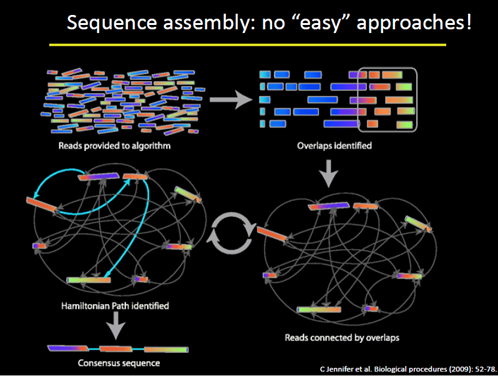
\includegraphics[width=0.6\textwidth]{Assembly.png}
\caption{}
\end{figure}

\begin{enumerate}
    \item They start from the reads obtained through sequencing and identify overlaps between them (this is performed by all algorithms).
    \item Once found, the order of the reads is defined by connecting reads by overlaps.
\end{enumerate}

In practice this is not always possible, due to many issues that occur, like:

\begin{itemize}
    \item multiple overlapping: there will be multiple overlapping of the same reads. Sometimes this is just due to a high coverage, sometimes (frequently) there may be different locations in the genomes that are matching, at least partially, our reads.
    \item partial matches, ecc.
\end{itemize}

One possible solution would be to \textbf{keep track of all possible matches} (overlaps) and then try to reconstruct the sequence. One way to represent the possible overlaps between reads is by using a \textbf{graph} in which the nodes represent the reads and the edges represent the connections between the reads that are overlapping in some way. 
Then, a \textbf{mathematical algorithm} is needed to find a solution in this very intricate network. 
Many assembly algorithms are available, and they are all based on this idea. For this reason, we always end up with multiple copies of genomes, not just one. 
Also, the output is almost never the full genome, but pieces of the genome, \textbf{multiple contigs}. Ideally, we could close the genome, but this is not possible just with short-read sequencing; other experiments are needed. By default, assembly is done in this way and gives a good representation of the genome, but not complete. Some quality control is also needed, especially to detect contamination.

The \textbf{general pipeline} for sequence assembly consists in a few steps:
\begin{enumerate}
    \item Find overlapping reads.
    \item Merge the 'good pairs' of reads into longer \textbf{contigs}. A contig is a contiguous sequence formed by several overlapping reads with no gaps.
    \item Link contigs to form \textbf{scaffolds} (or supercontigs), which are ordered and oriented sets of contigs. Scaffold assembly usually exploits mate pairs (which allows to link different contigs together, even if the information in the middle is not completely known). Mate pairs, also called long-insert paired-end reads (LIPERs), are a kind of read obtained from paired-end sequencing which can pair reads across greater distances. Scaffolds do contain gaps, but at least the order of the contigs is known and helps to reconstruct the whole genome. 
    \item Derive consensus sequence. Sometimes we have multiple scaffolds and the consensus sequence is the set of all scaffolds representing the genome or the chromosome that is being reconstructed.
\end{enumerate}

Finding the order of contigs is not easy and different approaches are used, hence scaffolding is usually a quite time-consuming operation. The aim would be to try to close the genome; for this purpose, some additional experiments could be needed. For example, one could use PCR to try to clone pieces between two contigs.
In microbial genomics, assembly usually finishes at the contig step. Contigs contained in the output files allow to define the genes present in the genome (for this goal, the order is not fundamental), whereas the position of genes in the genome is more difficult to study.
\textbf{What are mate pairs?} - Mate pair library preparation process
%From https://emea.illumina.com/science/technology/next-generation-sequencing/mate-pair-sequencing.html#:~:text=Introduction%20to%20Mate%20Pair%20Sequencing,Identification%20of%20complex%20genomic%20rearrangements
Following DNA fragmentation, the DNA fragments are end-repaired with labeled dNTPs. The DNA fragments are \textbf{circularized}, and non-circularized DNA is removed by digestion. Circular DNA is fragmented, and the labeled fragments (corresponding to the ends of the original DNA ligated together) are affinity-purified. Purified fragments are end-repaired and ligated to Illumina paired-end sequencing adapters.
Additional sequences complementary to the flow cell oligonucleotides are added to the adapter sequence with tailed PCR primers. The final prepared libraries consist of short fragments made up of two DNA segments that were originally separated by several kilobases. These libraries are ready for paired-end cluster generation, followed by sequencing utilizing an Illumina next-generation sequencing (NGS) system.
Combining data generated from mate pair library sequencing with that from short-insert paired-end reads provides a powerful combination of read lengths for maximal sequencing coverage across the genome.

\section{Feasibility of sequence assembly}

Doing a full assembly is considered to be impossible from a computational point of view. It is completely infeasible (NP hard), cannot be finished in a reasonable time, regardless the computational resources available. So technically assembly is impossible, differently from mapping, which is feasible. 
Read length $\xrightarrow[]{}$ important for reconstructing the whole sequence
Coverage $\xrightarrow[]{}$ many reads but impossible to assemble.

\subsection{Last year exercise}

As an example of the assembly process and of the aspects that might be important, students were asked to reconstruct a piece of English text which was previously fragmented.

\begin{figure}[h]
\centering
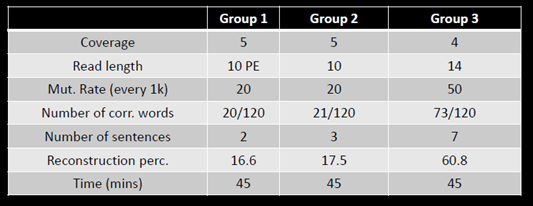
\includegraphics[width=0.6\textwidth]{Feasibility.png}
\caption{}
\end{figure}

Group 3 was the winner (highest percentage of reconstruction), despite having a lower coverage and a higher error rate, indicating that the length of the reads was very important. Without long-enough reads it was impossible to assemble sentences, going out of the repetitive regions of the text.
Knowing the characteristics of the sequence reads ('the language') might also help assembly. Eg. knowing that some sequences are just artifacts.

\subsection{Merging overlapping reads}

Basic principle: the strongest the similarity between the end of one read and the beginning of another the highest the likelihood the reads are coming from the same overlapping sequence region.
When overlapping reads, we must maximize the length of the overlap but also accuracy. Of course, since sequencing is not perfect, errors will happen. So again, we must find a score for the overlap. The fact that two reads are not perfectly overlapping can be due to different reasons:

\begin{itemize}
    \item they are not really contiguous (just similar sequences inside the genome). We should be able to distinguish between the two (not easy).
    \item Sequencing error/noise
    \item Diploid genome or multiple copy genomes: sometimes sequences coming from 2 different chromosomes; they are similar but not contiguous and this increases the difficulty.
\end{itemize}

\subsection{Overlap graphs}

As said, one way to represent reads overlaps is by using graphs. 
In an overlap graph, each read is a node, each overlap is an edge between two nodes, representing the two overlapping reads. Edges are directed: indicating that the final part of the first sequence matches the initial part of the second sequence. Directed graphs are very common in biology, for example to describe binding between proteins, or other biological functions.
Different overlaps can have different "strengths", based on the score of the overlap, so to each node we can also associate a weight.
Graphs are ideally cyclic, since in theory most organisms' DNAs are circular. So we could have the last read matching the first one. However, sometimes cycles are just due to random overlapping or to the presence of repeats. Those problems must be resolved in the mathematical object.
\textbf{The problem of the repeats} is a key aspect in bacterial genomics since bacterial genomes have many regions with repeats. Also, as we previously saw, short reads are the default sequencing technology for bacteria, and this increases the difficulty in assembly.

\begin{figure}[h]
\centering
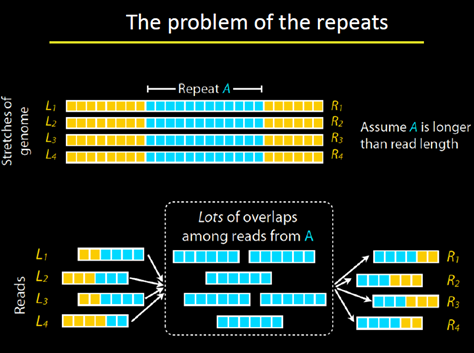
\includegraphics[width=0.6\textwidth]{Repeats.png}
\caption{Example of genome with repeats}
\end{figure}

If the read length is not long at least the length of the repeat, we will never be able to resolve this. The read that matches a part of the repeat and a part of the non-repeated region will be known, but for all reads that are inside the repeated region it will be impossible to define how long these regions are. There will be a lot of cycles and connecting the 2 non repeated parts won't be possible.
By knowing the \textbf{coverage} we can try to solve at least partially the problem. If we know that all the genes have a coverage of 10x for example, we could assume that the repeated part has a 10x coverage too and we could define a length for this region proportional to the expected coverage.
This is however a bit risky: repeated regions are also problematic for the sequencing machine, so there could be a skew in coverage for these regions.
The \textbf{safest idea} would be to \textbf{stop the contig} before the repetitive region (A) and start it again after it. Some assemblers will try to solve these repetitive regions and might produce a wrong contig. Hence, if we try to minimize the number of contigs produced (to obtain longer genome sequences) we might end up having wrong contigs (without even knowing it).
\textbf{Long reads} are the ultimate solution for this problem (they have many errors but represent a backbone on which to do the assembly).
With overlap graphs, which are not what assemblers are using right now, we can lead to having wrong contigs. The sides of regions containing repeats (mix of yellow and light-blue seen before) will overlap pretty good and will be considered as consequential in the sequence, discarding the repeated sequence in the middle. This will produce a wrong contig, in which fragments are considered to be \textbf{closer} than they are in reality. A solution could be to put many Ns in between and to keep track of the fact that the sequence is not reliable.
Some hints of the presence of repeated regions can be given by:

\begin{itemize}
    \item Coverage: we could see a region with a much higher coverage, which might contain actually repeats that were wrongly assembled.
    \item Paired-end: we could notice that the pairs over repeated regions have a shorter insert size than they should have. With long paired end sequencing we could also try to estimate the length of the regions with repeats.
\end{itemize}

\section{How to solve an overlapping graph?}

\begin{figure}[h]
\centering
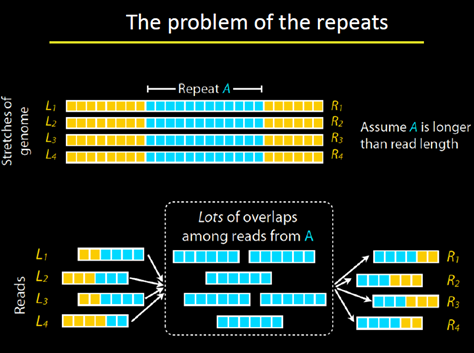
\includegraphics[width=0.6\textwidth]{Repeats.png}
\caption{}
\end{figure}

In this graph we have five known reads. Overlaps of length 1 are also present, usually not considered.
A possible ideal solution would be to use \textbf{Hamiltonian paths}. 
Hamiltonian paths are the paths touching all connected nodes once, so they provide all possible solutions. Then, how do we define which is the best one? We choose the one that maximizes the length of the overlaps. 
This problem however will explode, it implies too many possibilities. It is equivalent to the shortest common superstring (SCS) problem, and it is NP-hard = not feasible.
Another solution what be to use a \textbf{greedy approach}, which maximizes each choice, by following these steps:

\begin{enumerate}
    \item Randomly select a starting point/node.
    \item Select the connected node with maximum overlap as the next visitor.
\end{enumerate}

As always, the greedy approach will provide the best local solution, which might not be the best global solution.

\section{Graph simplification operations}

A practical trick that could be used to solve the graph, and to minimize the number of operations which must be performed (in an attempt to make it feasible), is to simplify it.
Simplification operations include:

\begin{itemize}
    \item Merging consecutive nodes: if among more reads there is only one possible path, we can just merge those reads, without losing information. So, nodes that are sequentially connected only with each other are linked together.
    \item  Remove dead ends: if some reads are branching from a path toward a dead-end, we can remove them. 
\end{itemize}
Here we may lose some information since the removed path could be the right one.
Assembly by overlap graphs has several problems:

\begin{itemize}
    \item It is problematic when dealing with repeats: maximizing the overall weight will produce wrong assemblies.
    \item It is not tractable: finding the optimal solution is not computationally feasible.
\end{itemize}

Overlap graphs can work to some extent, but now other algorithms are used in assemblers, like the de Bruijn Grpahs (DBG) and the Overlap Layout Consensus (OLC).

\begin{figure}[h]
\centering
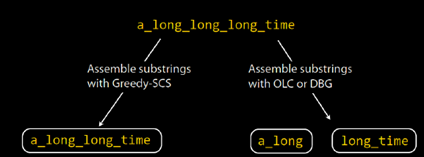
\includegraphics[width=0.6\textwidth]{DBG.png}
\caption{}
\end{figure}

As a simple example, in the case of the DBG, this problem would be splitted into 2 contigs, which is actually the best solution: better to have 2 right contigs, instead of 1 wrong contig.

\subsection{De Brujin graph assembly}

\begin{figure}[h]
\centering
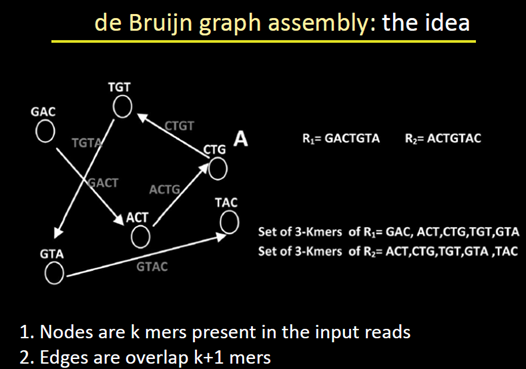
\includegraphics[width=0.6\textwidth]{DBGAssembly.png}
\caption{}
\end{figure}

On this graph the nodes are not the reads but the k-mers present in the input reads (with k smaller that the read-length). We define the length of k-mers length in advance and create all combinations of k-mers for each read, for example for reads R1 and R2. Clearly there will be some overlap, some k-mers will be present in both sequences, but in the graph there will be only one copy of them.
Hence, the nodes will be the \textbf{unique k-mers} present in the reads, the edges are the \textbf{overlaps} of the k-mers of length k+1 from the 2 sequences.
Then, instead of using Hamiltonian paths touching the nodes, we use \textbf{Eulerian paths}. 
Those are paths in which all edges are visited, each edge exactly once. From a computationally point of view, they can be found much more efficiently than Hamiltonian paths (no explosion of search space).
Other advantages: 

\begin{itemize}
    \item if we have a k-mer of length 3, we cannot have a huge amount of nodes, but 4\textsuperscript{3} possibilities. So the set of nodes will not be too big compared to the number of reads. With k = 3 $\xrightarrow[]{}$ huge amount of overlaps hence edges. But with longer k-mers (eg. 15) there will be a good trade off between the number of nodes and the number of edges.
    \item Cleaning reads: we can avoid putting in the k-mers that appear only once in a genome with a lot of coverage and are therefore the result of sequencing errors (otherwise the number of nodes would increase a lot).
    \item The de Bruijn graphs seem to be bigger sometimes, but they are not. With the de Bruijn graph the paths are more linear, there are less possibilities of wrong cycles. 
\end{itemize}

\subsection{Scaffolding}

\begin{figure}[h]
\centering
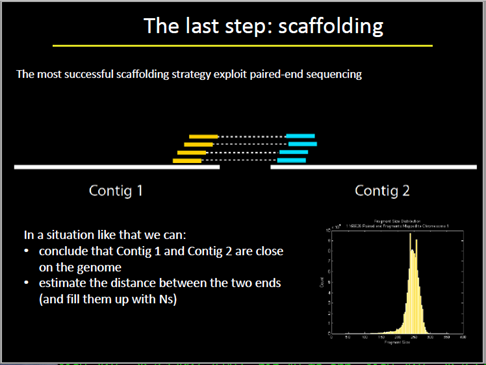
\includegraphics[width=0.6\textwidth]{Scaffolding.png}
\caption{}
\end{figure}

Scaffolding can be done with paired-end sequencing or with the estimation of the coverage. 
The fragment size in this case was 250 bp on average and with a Gaussian distribution like that one we can put an optimized number of Ns between the 2 contigs (not perfect, but connected). 
Doing it for all contigs leads again to a very complex situation.
Problems: If the end of a contig matches the middle of another one in paired-end sequencing, there might be a mistake. Either the contig must be splitted because the overlaps are wrong, or the two matches are wrong.

\subsection{Evaluating assemblies}

The \textbf{N50} is the size of a set of entities (e.g., contigs or scaffolds) which represents the largest entity E such that at least half of the total size of the entities is contained in entities larger than E.
Kind of a weighted median. For example, if we have a collection of contigs with sizes 7, 4, 3, 2, 2, the N50 is 4 because. 
(4 or more must be equal to what is 4 or less: 7+4 = 11, 4+2+2+3 = 11. Value in the middle for which the total length above and below is equal).
Long contigs help to have a higher N50. 
Other definition: N50 length is the length ‘x’ such that 50$\%$ of the sequence is contained in contigs of length x or greater. X must be the length of a real contigs, not just a number.
One long read = perfect N50 but might be wrong, we might check other characteristics. Eg. we can look at what the genes are coding for (is there at least a gene that codes for ribosomes? if not, wrong).

\begin{figure}[h]
\centering
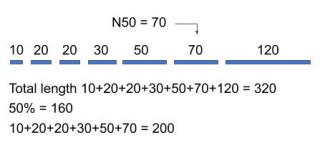
\includegraphics[width=0.6\textwidth]{Evalueate.png}
\caption{}
\end{figure}
